\chapter{HASIL DAN PEMBAHASAN}
\label{hasil-dan-pembahasan}
Bangunan yang dijadikan objek penelitian adalah \textit{climate chamber} DTNTF FT UGM. Dalam bab ini, akan dibahas mengenai hasil perancangan sistem kontrol sesuai dengan langkah-langkah yang dijelaskan pada Bab IV.

\section{Pengambilan Data Simulasi IES-VE}

\subsection{Kondisi \textit{Climate Chamber}}

\begin{figure}[!h]
	\centering
	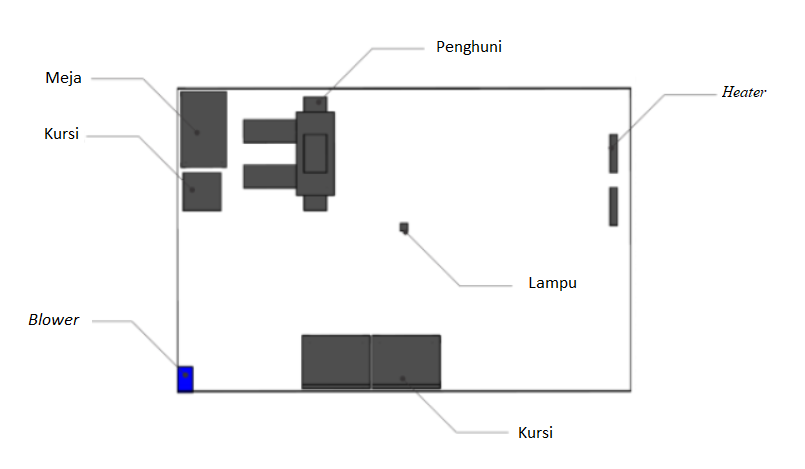
\includegraphics[width=1\textwidth]{figures/KondisiChamber}
	\caption{Posisi Komponen-Komponen di dalam \textit{Climate Chamber}}
	\label{fig:5:KondisiChamber}
\end{figure}
%\vspace{1em}

Climate chamber memiliki ukuran 3m $\times$ 2m $\times$ 3m (p $\times$ l $\times$ t). Komponen-komponen di dalam climate chamber terdiri dari meja, kursi, blower, penghuni, lampu, heater, dan AC.\\

\begin{figure}[!h]
	\centering
	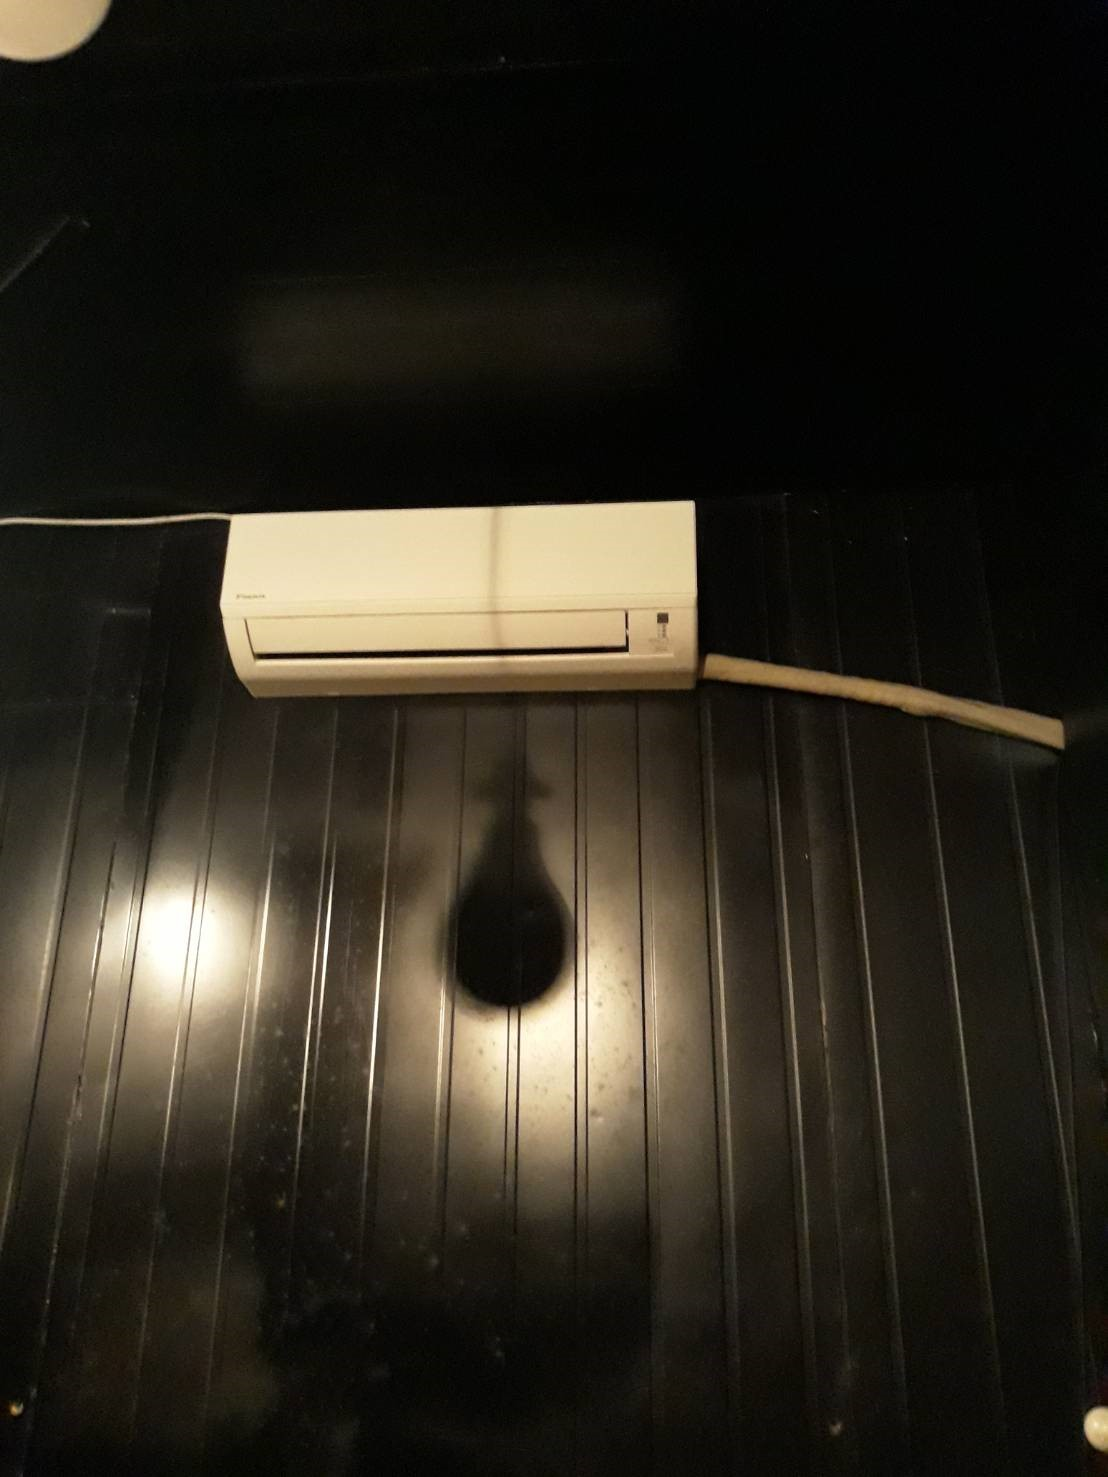
\includegraphics[width=0.75\textwidth]{figures/AC}
	\caption{Perangkat AC}
	\label{fig:5:AC}
\end{figure}
%\vspace{1em}

\begin{figure}[!h]
	\centering
	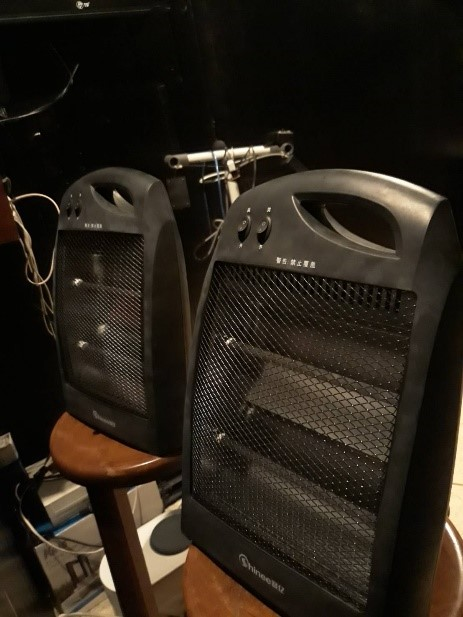
\includegraphics[width=0.5\textwidth]{figures/Heater}
	\caption{Perangkat Heater}
	\label{fig:5:Heater}
\end{figure}
%\vspace{1em}

Perangkat AC yang berada di dalam climate Chamber DTNTF UGM memiliki daya sebesar 2800W (1 PK). Perangkat AC mampu mengkondisikan lingkungan melalui aliran udara yang keluar. Maka dari itu, Perangkat AC sangatlah berpengaruh terhadap kondisi lingkungan termal di dalam ruangan. Tampak dari wujud perangkat AC dapat dilihat pada Gambar \ref{fig:5:AC}

Perangkat heater yang berada di dalam climate chamber memiliki daya sebesar 900W. Terdapat dua buah perangkat heater di dalam climate chamber. Semakin banyak perangkat heater yang aktif maka akan suhu udara akan menjadi semakin meningkat. Kenaikan rerata suhu udara yaitu sebesar $\pm1,9^\circ$C untuk setiap perangkat heater. Tampak dari wujud perangkat heater dapat dilihat pada Gambar \ref{fig:5:Heater}.

Selain faktor dari dalam \textit{climate chamber}, faktor dari luar ruangan \textit{climate chamber} pun secara tidak langsung mempengaruhi kondisi lingkungan termal \textit{climate chamber}. Diantaranya adalah suhu udara luar (\textit{dry bulb temperature}) dan intensitas radiasi matahari. Posisi harian matahari mempengaruhi perubahan nilai suhu udara luar dan intensitas radiasi matahari. Pada siang hari (posisi altitude matahari ketika berada tepat diatas \textit{climate chamber}) memberikan paparan radiasi matahari yang mengenai selubung bangunan. Hal ini menyebabkan kenaikan suhu di dalam \textit{climate chamber}. Kalor yang menembus selubung bangunan berbanding lurus dengan nilai U-value. Nilai U-Value pada selubung bangunan dapat dilihat pada Tabel \ref{tbl:5:UValue}.\\

\begin{table}[!h]
	\caption{U-Value Selubung Climate Chamber\cite{skripsiTanto}}
	\label{tbl:5:UValue}
	\centering
	% use packages: array
	\begin{tabular}{|p{5.7cm}|p{5cm}|}
		\hline
		\textbf{Selubung Climate Chamber} & \textbf{U-Value (W/m$^2$.K)} \\ \hline
		Dinding & 0,707 \\ \hline
		Atap & 1,996 \\ \hline 
		Lantai & 0,707 \\ \hline
	\end{tabular}
\end{table}

\subsection{Rancangan Skenario Pengambilan Data}
Rancangan skenario pada climate chamber menghasilkan kombinasi antara set AC dan jumlah heater ON. Set AC dikondisikan untuk menyala dari pukul 08:00 s.d. 17:00 dengan rentang nilai 16$^\circ$C - 30$^\circ$C. Set jumlah heater ON terbagi menjadi 3 kondisi, yaitu keduanya tidak menyala (berkode 0), salah satu menyala (berkode 1), dan keduanya menyala (berkode 2). Kombinasi tersebut menghasilkan 25 variasi skenario. Untuk variasi suhu luar dan intensitas radiasi matahari, penulis bersama Tanto sepakat untuk menggunakan 4 titik ekstrim bumi terhadap matahari yaitu pada tanggal 21 Maret, 21 Juni, 23 September dan 22 Desember. Kemudian kami melakukan simulasi disetiap titik tersebut dengan kombinasi set heater dan set AC seperti pada Gambar \ref{fig:5:HeaterAC}. Sehingga, total skenario yang dihasilkan dari kombinasi tersebut berjumlah 100 skenario.

\begin{figure}[!h]
	\centering
	
\includegraphics[width=0.65\textwidth]{figures/SkenarioData}
	\caption{Skenario Pengambilan Data}
	\label{fig:5:SkenarioData}
\end{figure}
%\vspace{1em}

\begin{figure}[!h]
	\centering
	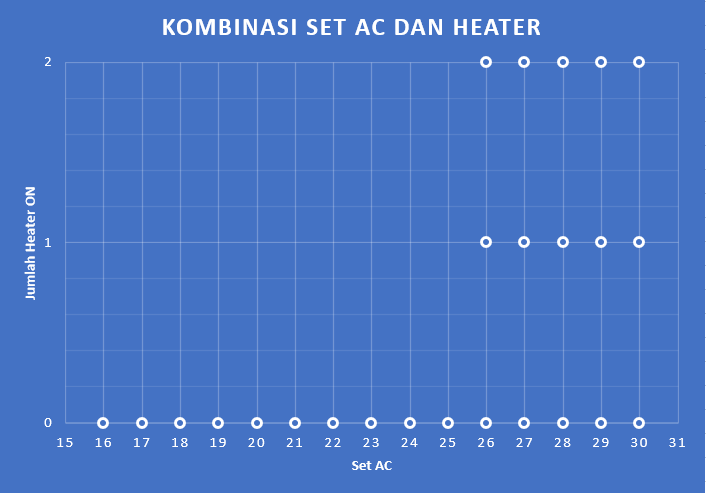
\includegraphics[width=0.5\textwidth]{figures/HeaterAC}
	\caption{Kombinasi SET AC dan Heater}
	\label{fig:5:HeaterAC}
\end{figure}
%\vspace{1em}

\subsection{Simulasi IES-VE}

Pada Gambar \ref{fig:5:SimulasiIESVE} penulis menunjukan salah satu hasi simulasi untuk skenario
SET AC 26$^\circ$C dan SET Heater ON 2 buah. Grafik yang ditampilkan terdiri dari 4
parameter yaitu suhu luar (To), intensitas radiasi matahari (RD), suhu udara ruang (Td), dan kelembapan relatif (RH).

\begin{figure}[!h]
	\centering
	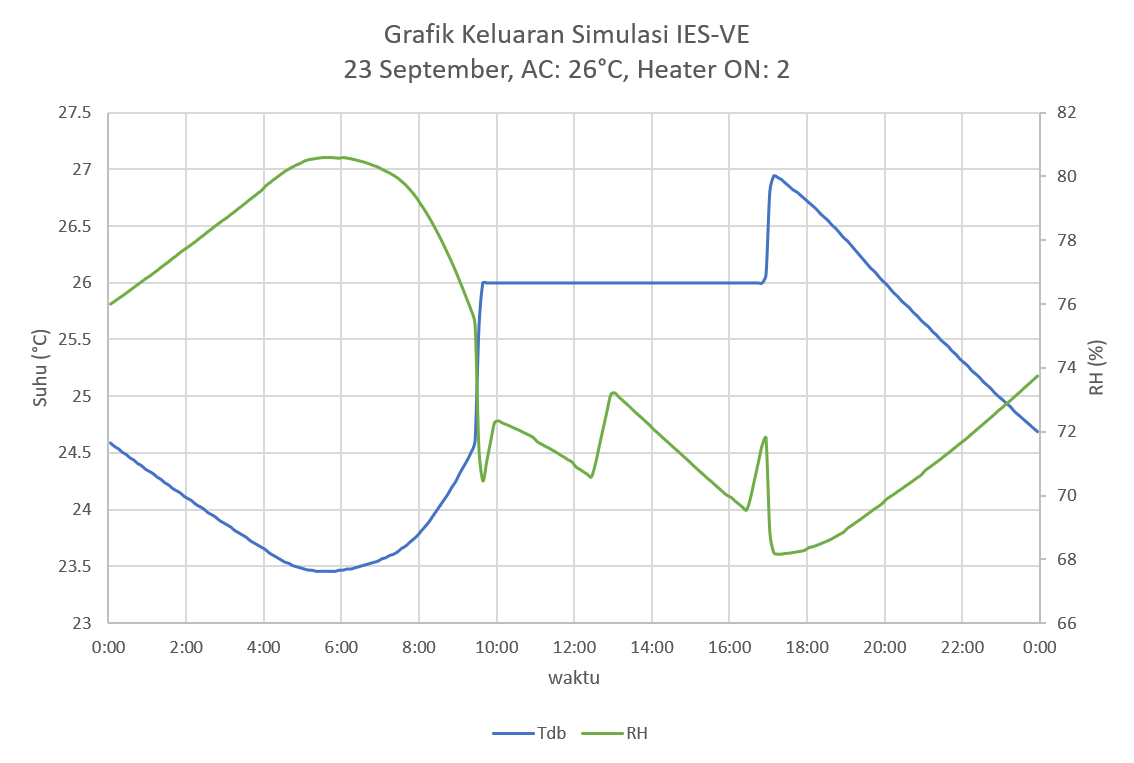
\includegraphics[width=0.8\textwidth]{figures/HasilSimulasiIESVE}
	\caption{Perangkat Heater}
	\label{fig:5:SimulasiIESVE}
\end{figure}
%\vspace{1em}

Skenario diatas dilakukan selama 24 jam dengan selang waktu pengambilan data selama 6 menit dimulai dari pukul 00:03 hingga 23:57. Selang waktu tersebut adalah waktu tersingkat yang dapat dilakukan pada software IES-VE 2019. Respon waktu suhu udara terhadap aktivasi AC tidak penulis perhitungkan dikarenakan secara fisis, respons transien termal pada bangunan cukup lama, sehingga hanya berfokus untuk meninjau nilai kesalahan keadaan-ajeg (\textit{steady-state error}).

\section{Pengembangan Model Plant JST}

Model Plant menggunakan model JST yang telah dibangun oleh Tri Hartanto\cite{skripsiTanto} sebagai model acuan dalam penelitian ini. Model tersebut kemudian dikembangan kembali untuk meningkatkan kinerjanya sebagai model \textit{plant}. \textit{Hyperparameter} yang digunakan Tri Hartanto pada pembangunan model plant JST ini dijelaskan pada Tabel \ref{tbl:5:NNPlantTanto}. Kinerja model dievaluasi dengan meninjau nilai MAE dari model tersebut.\\

\begin{table}[!h]
	\caption{Tabel Rancangan Model Plant JST\cite{skripsiTanto}}
	\label{tbl:5:NNPlantTanto}
	\centering
	% use packages: array
	\begin{tabular}{|p{5.7cm}|p{5cm}|}
		\hline
		\textbf{Nama Hyperparameter} & \textbf{Nilai Hyperparameter} \\ \hline
		Arsitektur & Feedforward Neural Network \\ \hline
		Pembagian Data & 50\% 25\% 25\% \\ \hline 
		Jumlah Layar Tersembunyi & 1 \\ \hline
		Jumlah Neuron pada Layar & [55] \\ \hline
		Fungsi Aktivasi Layar & Hyperbolic Tangent \\ \hline
		Algoritma Pembelajaran & Levenberg-Marquardt \\ \hline
		Mean Absolute Error (MAE) & Td: 0,59$^\circ$C ; RH: 5,44\% \\ \hline
		Mean Squared Error (MSE) & Td: 0,75$^\circ$C ; RH: 52,33\% \\ \hline
		Koefisien Korelasi (R) & Td: 96,23\% ; RH: 68,90\% \\ \hline
	\end{tabular}
\end{table}

%Tri Hartanto membangun model \textit{plant} dengan menggunakan data menyeluruh selama 24 jam. Pada penelitian ini penulis membangun model dengan menggunakan data selama jam operasional, yaitu pukul 07:00 s.d. 17:00. Hal ini dilakukan karena pada praktiknya \textit{climate chamber} digunakan untuk pengujian pada jam operasional tersebut. Hasil model \textit{plant} dengan penyesuaian data ini dapat dilihat pada Tabel \ref{tbl:5:NNPlantTanto2}.

\subsection{Variasi Pembagian Data} 

Variasi pembagiaan data dilakukan dengan membandingkan beberapa variasi pembagiaan data ke dalam 5 variasi. Kemudian kinerja dari setiap pembagian data dibandingkan dengan konfigurasi \textit{hyperparameter} pada \ref{tbl:5:NNPlantTanto}.

\begin{table}[h!]
	\caption{Daftar variasi pembagian data}
	\label{tbl:5:DataSplitting}
	\centering
	% use packages: array
	\begin{tabular}{|p{3cm}|p{3cm}|p{1.5cm}|p{1cm}|p{1.5cm}|p{1cm}|}
		\hline
		Pembagian Data   & Persentase Data \\ \hline
		Data Splitting 0 & (50\% 25\% 25\%)\\ \hline
		Data Splitting 1 & (60\% 20\% 20\%)\\ \hline
		Data Splitting 2 & (70\% 15\% 15\%)\\ \hline
		Data Splitting 3 & (80\% 10\% 10\%)\\ \hline
		Data Splitting 4 & (80\% 15\% 05\%)\\ \hline
		Data Splitting 5 & (85\% 10\% 05\%)\\ \hline
	\end{tabular}
\end{table}

\begin{figure}[!h]
	\centering
	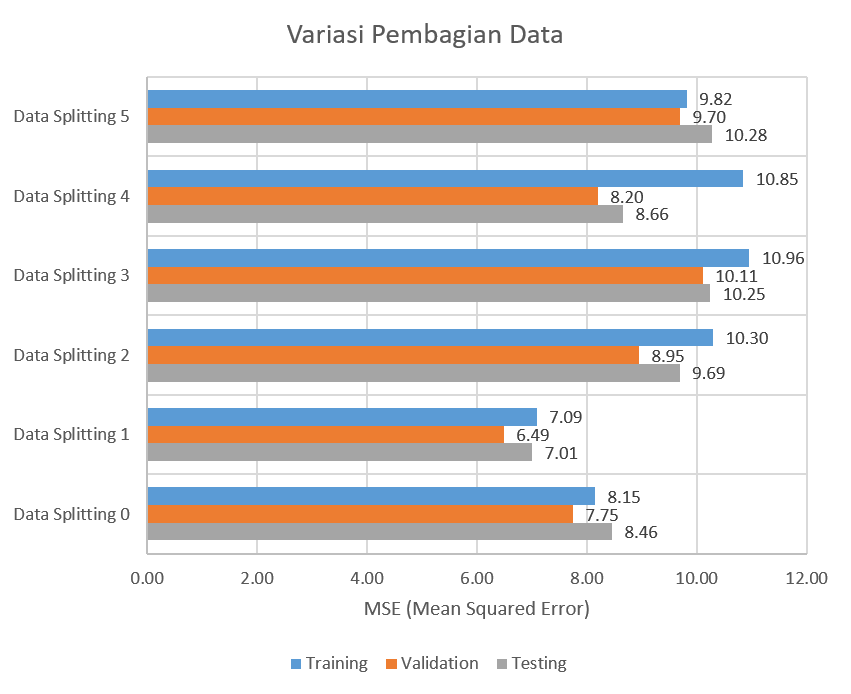
\includegraphics[width=0.9\textwidth]{figures/DataSplittingResult}
	\caption{Hasil Variasi Pembagian Data}
	\label{fig:5:DataSplittingResult}
\end{figure}

\begin{figure}[!h]
	\centering
	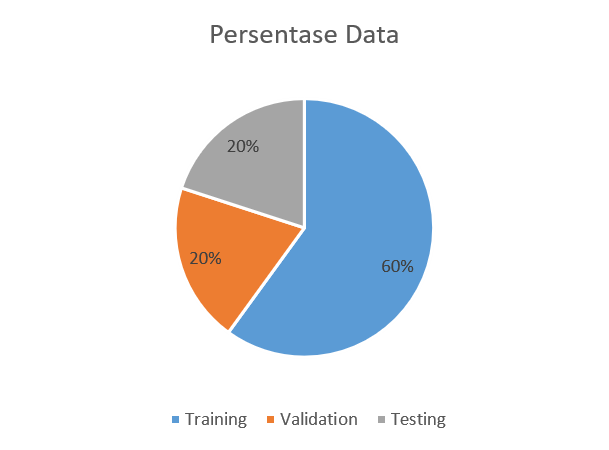
\includegraphics[width=0.75\textwidth]{figures/DataSplittingFinal}
	\caption{Pembagian Data yang digunakan}
	\label{fig:5:DataSplittingFinal}
\end{figure}
\vspace{1em}

Pada Tabel \ref{tbl:5:DataSplitting}, "Data Splitting 0" merupakan konfigurasi pembagian data yang digunakan oleh Tri Hartanto pada penelitian sebelumnya dalam membangun model plant JST. Pada tabel yang penulis sajikan, penulis menulis pembagian data dengan format 'Data Splitting n' dan '(x\% y\% z\%)' dimana n = nomor variasi, x = pembagian data pelatihan, y = pembagian data validasi, dan z = pembagian data pengujian. Pembagian data terbaik yang penulis gunakan yaitu pembagian data bernama "Data Splitting 4". Data dibagi menjadi 3 bagian, yakni 80\% data pelatihan, 15\% data validasi, dan 5\% data pengujian. Sehingga didapatkan rancangan terbaik penulis yang dirangkum pada Tabel \ref{tbl:5:NNPlantRidhan}.\\

\begin{table}[!h]
	\caption{Tabel Rancangan Model Plant JST Penulis}
	\label{tbl:5:NNPlantRidhan}
	\centering
	% use packages: array
	\begin{tabular}{|p{5.7cm}|p{5cm}|}
		\hline
		\textbf{Nama Hyperparameter} & \textbf{Nilai Hyperparameter} \\ \hline
		Arsitektur & Feedforward Neural Network \\ \hline
		Pembagian Data & 80\% 15\% 5\% \\ \hline 
		Jumlah Layar Tersembunyi & 1 \\ \hline
		Jumlah Neuron pada Layar & [55] \\ \hline
		Fungsi Aktivasi Layar & Hyperbolic Tangent \\ \hline
		Algoritma Pembelajaran & Levenberg-Marquardt \\ \hline
		Mean Absolute Error (MAE) & Td: 0,62$^\circ$C ; RH: 5,45\% \\ \hline
		Mean Squared Error (MSE) & Td: 0,82$^\circ$C ; RH: 54,45\% \\ \hline
		Koefisien Korelasi (R) & Td: 93,09\% ; RH: 71,44\% \\ \hline
	\end{tabular}
\end{table}

Dari pengembangan model plant JST ini, didapatkan rancangan yang lebih baik dari hasil kinerja rancangan sebelumnya. Dengan mengubah pembagiaan data dari 50\% 25\% 25\% ke 80\% 15\% 5\%, nilai MAE model untuk kelembapan relatif pun berubah menjadi sebesar 0,62$^\circ$C.

\section{Perancangan Sistem Kontrol JST}

Perancangan sistem kontrol dipilih dengan membandingkan kinerja dengan nilai \textit{steady-state error} dari 4 rancangan sistem kontrol berbasis jaringan saraf tiruan. Keempat rancangan sistem kontrol tersebut adalah sebagai berikut:
\begin{enumerate}
	\item Design I: NN Inverse Model Control
	\item Design II: NN Inverse Model Control umpan balik Variabel Manipulasi
	\item Design III: NN Inverse Model Control umpan balik Variabel Gangguan
	\item Design IV: NN Internal Model Control
\end{enumerate}

Kinerja dari keempat rancangan sistem kontrol diatas dapat diamati pada Gambar \ref{fig:5:ControllerComparisonTd} untuk suhu ruang dan Gambar \ref{fig:5:ControllerComparisonRH} untuk kelembapan relatif.

\begin{figure}[!h]
	\centering
	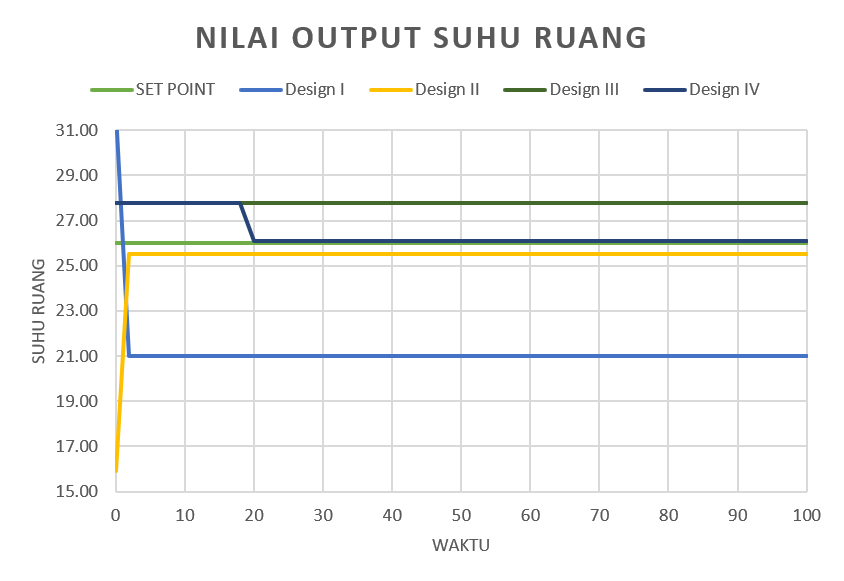
\includegraphics[width=0.9\textwidth]{figures/ControlSystemComparisonTd}
	\caption{Pembagian Data yang digunakan}
	\label{fig:5:ControllerComparisonTd}
\end{figure}

\begin{figure}[!h]
	\centering
	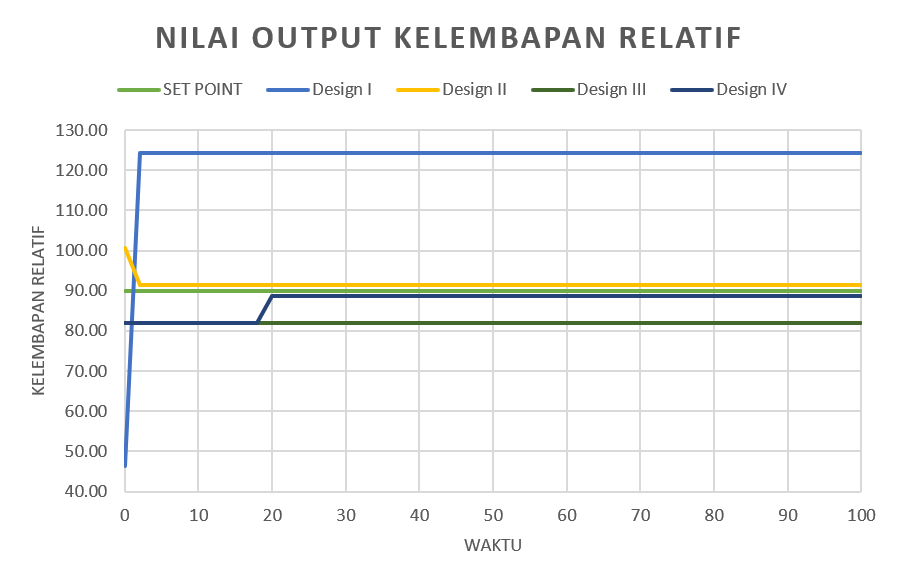
\includegraphics[width=0.9\textwidth]{figures/ControlSystemComparisonRH}
	\caption{Pembagian Data yang digunakan}
	\label{fig:5:ControllerComparisonRH}
\end{figure}
\vspace{1em}

Berdasarkan Gambar \ref{fig:5:ControllerComparisonTd} dan Gambar \ref{fig:5:ControllerComparisonRH}, dapat dilihat bahwa rancangan terbaik dengan nilai \textit{steady-state error} paling rendah adalah rancangan Design IV: NN Internal Model Control. Sehingga rancangan ini yang dipilih untuk digunakan sebagai sistem kontrol. 

NN Internal Model Control terdiri dari 3 komponen utama, yaitu: Plant, Emulator, dan Kontroler. Emulator dibangun dari model umpan maju JST (\textit{NN Forward Model}) dan kontroler dibangun dari model umpan balik JST (\textit{NN Inverse Model}). Blok diagram untuk Emulator dapat dilihat pada Lampiran \ref{fig:C:NNForwardModelDesign} dan untuk Kontroler dapat dilihat pada Lampiran \ref{fig:C:NNInverseModelDesign}.

\subsection{Kinerja Emulator JST}

Emulator JST dibangun menyerupai rancangan model plant JST. Perbedaannya berada pada masukan dan keluaran dari arsitektur JST. Emulator juga menggunakan nilai Output Plant sebelumnya sebagai masukan untuk memprediksi nilai Output Plant pada saat ini. Hasil kinerja emulator JST ini dijabarkan pada Tabel \ref{tbl:5:NNEmulator}

\begin{table}[!hbt]
	\caption{Tabel Rancangan Emulator JST (\textit{NN Forward Model})}
	\label{tbl:5:NNEmulator}
	\centering
	% use packages: array
	\begin{tabular}{|p{5.7cm}|p{5cm}|}
		\hline
		\textbf{Nama Hyperparameter} & \textbf{Nilai Hyperparameter} \\ \hline
		Arsitektur & Feedforward Neural Network \\ \hline
		Pembagian Data & 80\% 15\% 5\% \\ \hline 
		Jumlah Layar Tersembunyi & 1 \\ \hline
		Jumlah Neuron pada Layar & [55] \\ \hline
		Fungsi Aktivasi Layar & Hyperbolic Tangent \\ \hline
		Algoritma Pembelajaran & Levenberg-Marquardt \\ \hline
		Mean Absolute Error (MAE) & Td: 0,51$^\circ$C ; RH: 1,43\% \\ \hline
		Mean Squared Error (MSE) & Td: 0,49$^\circ$C ; RH: 5,91\% \\ \hline
		Koefisien Korelasi (R) & Td: 96,38\% ; RH: 97,79\% \\ \hline
	\end{tabular}
\end{table}

\subsection{Kinerja Kontroler JST}

Kontroler JST dibangun dengan proses invers dari model plant JST. Pada proses pelatihan JST, dilakukan pengskalaan terhadap semua input JST menggunakan metode \textit{Min Max Scaling} kecuali variabel delay umpan masuk SET AC dan SET Heater. Pengskalaan bertujuan untuk meningkatkan kinerja JST menjadi optimal dengan menyamakan rentang nilai dan besar satuan dari setiap variabel (berupa rentang nilai dari 0 hingga 1). Masing-masing variabel diubah menjadi skala satuan dengan melakukan transformasi data secara statistik. Data dari setiap variabel akan dikurangi dengan nilai minimum variabel tersebut yang dikemudian dibagi oleh selisih dari nilai maksimum dan nilai minimum variabel tersebut. Secara lengkap dapat dirumuskan pada persamaan berikut:
\begin{equation} \label{eq:5:MinMaxScaler}
z = \frac{x_i - min(x)}{max(x) - min(x)}
\end{equation}

Rancangan kontroler JST mirip dengan rancangan model plant JST. Perbedaannya hanyalah pada jumlah neuron pada \textit{hidden layer} yang berjumlah 52 neuron. Hasil kinerja dari kontroler JST ini dapat dilihat pada Tabel \ref{tbl:5:NNControler}.

\begin{table}[!h]
	\caption{Tabel Rancangan Kontroler JST (\textit{NN Inverse Model})}
	\label{tbl:5:NNControler}
	\centering
	% use packages: array
	\begin{tabular}{|p{5.7cm}|p{5cm}|}
		\hline
		\textbf{Nama Hyperparameter} & \textbf{Nilai Hyperparameter} \\ \hline
		Arsitektur & Feedforward Neural Network \\ \hline
		Pembagian Data & 80\% 15\% 5\% \\ \hline 
		Jumlah Layar Tersembunyi & 1 \\ \hline
		Jumlah Neuron pada Layar & [52] \\ \hline
		Fungsi Aktivasi Layar & Hyperbolic Tangent \\ \hline
		Algoritma Pembelajaran & Levenberg-Marquardt \\ \hline
		Mean Absolute Error (MAE) & AC: 0,23$^\circ$C ; HT: 0,00 \\ \hline
		Mean Squared Error (MSE) & AC: 4,85$^\circ$C ; HT: 0,00 \\ \hline
		Koefisien Korelasi (R) & AC: 98,41\% ; HT: 99,64\% \\ \hline
	\end{tabular}
\end{table}

\hfill\break
\hfill\break

\subsection{Kinerja Sistem Kontrol JST}

Sistem kontrol terpilih diuji dengan 3 variasi kombinasi SET POINT. Kombinasi terdiri dari SET POINT untuk variabel yang diingikan dan variabel gangguan. Ketiga variasi tersebut adalah sebagai berikut:
\begin{enumerate}
	\item SP1
	\begin{table}[!h]
		\caption{Nilai Kombinasi SET POINT SP1}
		\label{tbl:5:SP1Combination}
		\centering
		% use packages: array
		\begin{tabular}{|l|c|}
			\hline
			\textbf{Variabel} & \textbf{SET Point} \\ \hline
			Suhu Ruang (Td) & 26$^\circ$C          \\ \hline
			Kelembapan Relatif (RH) & 90\%         \\ \hline
			Suhu Luar (To) & 27$^\circ$C           \\ \hline
			Radiasi Matahari (RD) & 400 W/m$^2$    \\ \hline
		\end{tabular}
	\end{table}
	
	\item SP2
	\begin{table}[!h]
		\caption{Nilai Kombinasi SET POINT SP2}
		\label{tbl:5:SP2Combination}
		\centering
		% use packages: array
		\begin{tabular}{|l|c|}
			\hline
			\textbf{Variabel} & \textbf{SET Point} \\ \hline
			Suhu Ruang (Td) & 27$^\circ$C          \\ \hline
			Kelembapan Relatif (RH) & 85\%         \\ \hline
			Suhu Luar (To) & 27$^\circ$C           \\ \hline
			Radiasi Matahari (RD) & 400 W/m$^2$    \\ \hline
		\end{tabular}
	\end{table}
	
	\item SP3
	\begin{table}[!h]
		\caption{Nilai Kombinasi SET POINT SP3}
		\label{tbl:5:SP3Combination}
		\centering
		% use packages: array
		\begin{tabular}{|l|c|}
			\hline
			\textbf{Variabel} & \textbf{SET Point} \\ \hline
			Suhu Ruang (Td) & Step 26$^\circ$C -> 27$^\circ$C \\ \hline
			Kelembapan Relatif (RH) & Step 90\% -> 85\% \\ \hline
			Suhu Luar (To) & 27$^\circ$C           \\ \hline
			Radiasi Matahari (RD) & 400 W/m$^2$    \\ \hline
		\end{tabular}
	\end{table}
\end{enumerate}

\subsubsection{SET POINT SP1}

Kombinasi SET Point dapat dilihat pada Tabel \ref{tbl:5:SP1Combination}. Hasil dari simulasi simulink dapat dilihat pada Gambar \ref{fig:5:SimulinkSP1Td} dan Gambar \ref{fig:5:SimulinkSP1RH}. Pada Gambar \ref{fig:5:SimulinkSP1Td} dan Gambar \ref{fig:5:SimulinkSP1RH} dapat dilihat bahwa nilai \textit{steady-state error} sistem kontrol cukup kecil. Nilai \textit{steady-state error} dari simulasi ini dapat dilihat pada Tabel \ref{tbl:5:SP1Ess}. Grafik dari hasil simulasi dapat dilihat pada Gambar \ref{fig:5:SimulinkSP1Td} untuk Suhu Ruang dan Gambar \ref{fig:5:SimulinkSP1RH} untuk Kelembapan Relatif. Kontroler mengeluarkan nilai \textit{Manipulated Variable} yang ditunjukkan oleh Gambar \ref{fig:5:SimulinkSP1AC} dan Gambar \ref{fig:5:SimulinkSP1HT}.\\

\begin{table}[!h]
	\caption{Hasil Simulasi Sistem Kontrol SP1}
	\label{tbl:5:SP1Ess}
	\centering
	% use packages: array
	\begin{tabular}{|l|c|c|c|}
		\hline
		\textbf{Variabel} & \textbf{SET Point} & \textbf{Output Plant} & \textbf{Steady-State Error}\\ \hline
		Suhu Ruang (Td) & 26$^\circ$C & 26,09$^\circ$C & 0,09$^\circ$C \\ \hline
		Kelembapan Relatif (RH) & 90\% & 88,76\% & 1,24\% \\ \hline
	\end{tabular}
\end{table}
\hfill\break

\begin{figure}[!h]
	\centering
	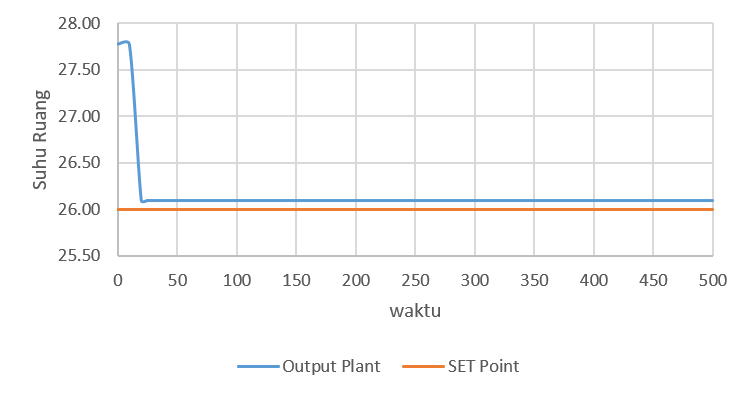
\includegraphics[width=0.75\textwidth]{figures/SimulinkSP1Td}
	\caption{Hasil Simulasi Sistem Kontrol untuk Suhu Ruang SP1}
	\label{fig:5:SimulinkSP1Td}
\end{figure}

\begin{figure}[!h]
	\centering
	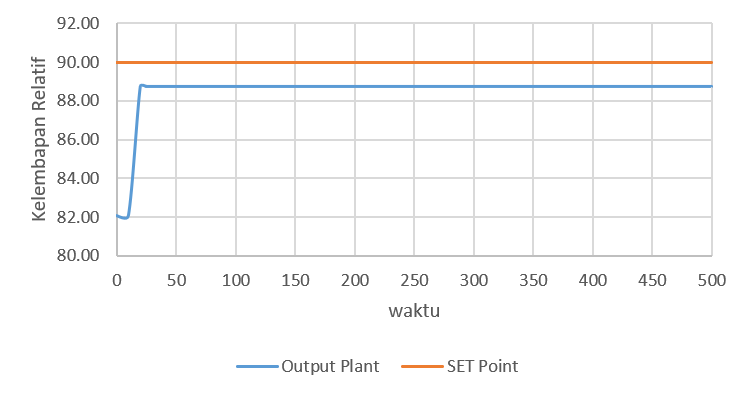
\includegraphics[width=0.75\textwidth]{figures/SimulinkSP1RH}
	\caption{Hasil Simulasi Sistem Kontrol untuk Kelembapan Relatif SP1}
	\label{fig:5:SimulinkSP1RH}
\end{figure}

\begin{figure}[!h]
	\centering
	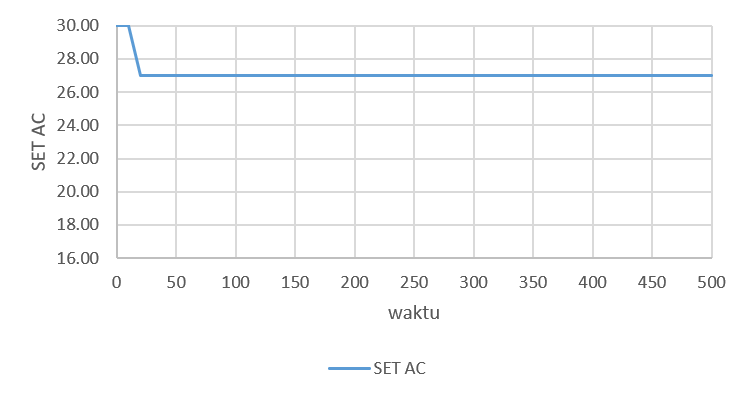
\includegraphics[width=0.75\textwidth]{figures/SimulinkSP1AC}
	\caption{Nilai MV SET AC SP1}
	\label{fig:5:SimulinkSP1AC}
\end{figure}

\begin{figure}[!h]
	\centering
	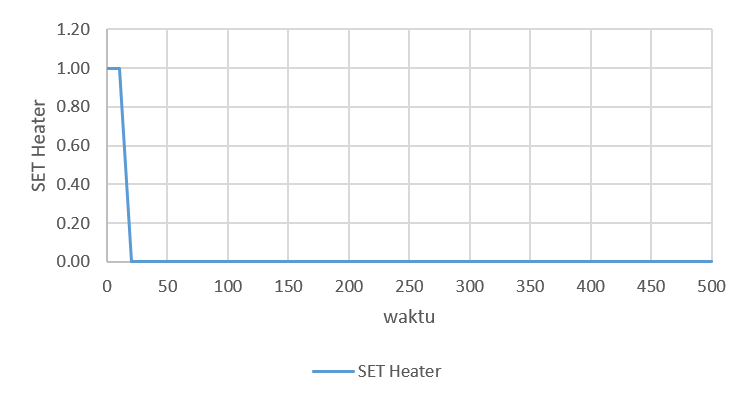
\includegraphics[width=0.75\textwidth]{figures/SimulinkSP1HT}
	\caption{Nilai MV SET Heater SP1}
	\label{fig:5:SimulinkSP1HT}
\end{figure}

\subsubsection{SET POINT SP2}

Kombinasi SET Point dapat dilihat pada Tabel \ref{tbl:5:SP2Combination}. Hasil dari simulasi simulink dapat dilihat pada Gambar \ref{fig:5:SimulinkSP2Td} dan Gambar \ref{fig:5:SimulinkSP2RH}. Pada Gambar \ref{fig:5:SimulinkSP2Td} dan Gambar \ref{fig:5:SimulinkSP2RH} dapat dilihat bahwa nilai \textit{steady-state error} sistem kontrol cukup kecil. Nilai \textit{steady-state error} dari simulasi ini dapat dilihat pada Tabel \ref{tbl:5:SP2Ess}. Grafik dari hasil simulasi dapat dilihat pada Gambar \ref{fig:5:SimulinkSP2Td} untuk Suhu Ruang dan Gambar \ref{fig:5:SimulinkSP2RH} untuk Kelembapan Relatif. Kontroler mengeluarkan nilai \textit{Manipulated Variable} yang ditunjukkan oleh Gambar \ref{fig:5:SimulinkSP2AC} dan Gambar \ref{fig:5:SimulinkSP2HT}.\\

\begin{table}[!h]
	\caption{Hasil Simulasi Sistem Kontrol SP2}
	\label{tbl:5:SP2Ess}
	\centering
	% use packages: array
	\begin{tabular}{|l|c|c|c|}
		\hline
		\textbf{Variabel} & \textbf{SET Point} & \textbf{Output Plant} & \textbf{Steady-State Error}\\ \hline
		Suhu Ruang (Td) & 27$^\circ$C & 27,09$^\circ$C & 0,09$^\circ$C \\ \hline
		Kelembapan Relatif (RH) & 85\% & 86,14\% & 1,14\% \\ \hline
	\end{tabular}
\end{table}
\hfill\break

\begin{figure}[!h]
	\centering
	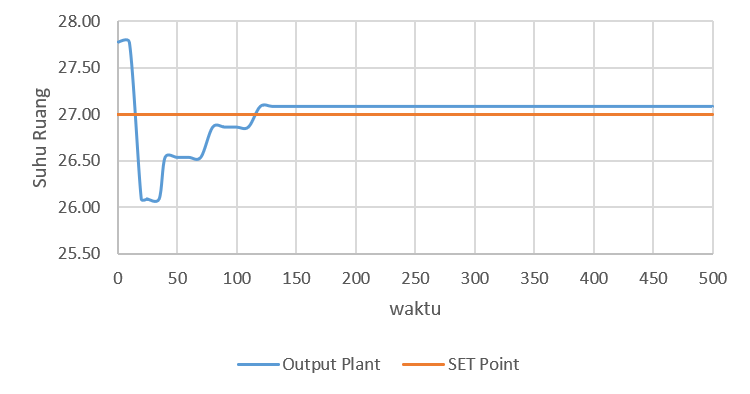
\includegraphics[width=0.75\textwidth]{figures/SimulinkSP2Td}
	\caption{Hasil Simulasi Sistem Kontrol untuk Suhu Ruang SP2}
	\label{fig:5:SimulinkSP2Td}
\end{figure}

\begin{figure}[!h]
	\centering
	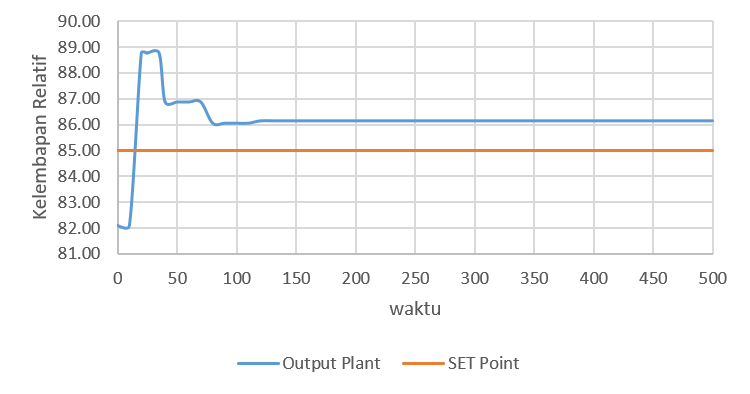
\includegraphics[width=0.75\textwidth]{figures/SimulinkSP2RH}
	\caption{Hasil Simulasi Sistem Kontrol untuk Kelembapan Relatif SP2}
	\label{fig:5:SimulinkSP2RH}
\end{figure}

\begin{figure}[!h]
	\centering
	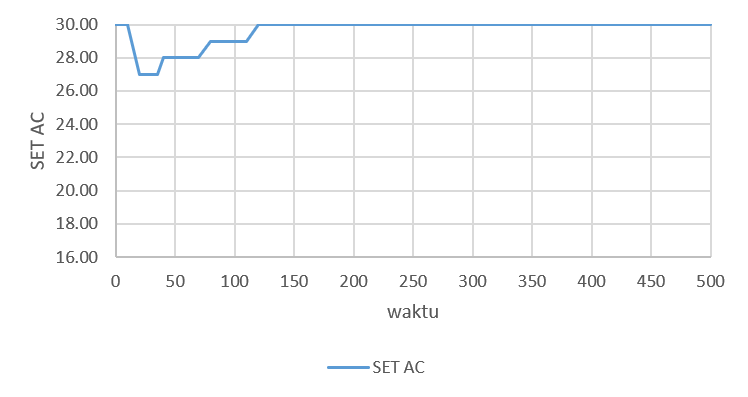
\includegraphics[width=0.75\textwidth]{figures/SimulinkSP2AC}
	\caption{Nilai MV SET AC SP2}
	\label{fig:5:SimulinkSP2AC}
\end{figure}

\begin{figure}[!h]
	\centering
	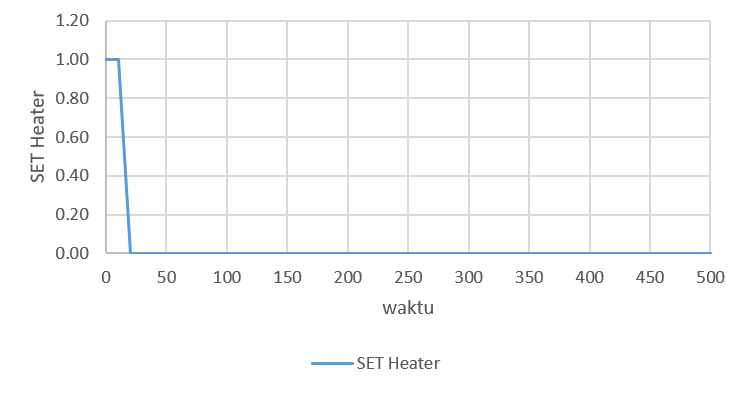
\includegraphics[width=0.75\textwidth]{figures/SimulinkSP2HT}
	\caption{Nilai MV SET Heater SP2}
	\label{fig:5:SimulinkSP2HT}
\end{figure}

\subsubsection{SET POINT SP3}

Kombinasi SET Point dapat dilihat pada Tabel \ref{tbl:5:SP3Combination}. Hasil dari simulasi simulink dapat dilihat pada Gambar \ref{fig:5:SimulinkSP3Td} dan Gambar \ref{fig:5:SimulinkSP3RH}. Pada Gambar \ref{fig:5:SimulinkSP3Td} dan Gambar \ref{fig:5:SimulinkSP3RH} dapat dilihat bahwa nilai \textit{steady-state error} sistem kontrol cukup kecil. Nilai \textit{steady-state error} dari simulasi ini dapat dilihat pada Tabel \ref{tbl:5:SP3Ess}. Grafik dari hasil simulasi dapat dilihat pada Gambar \ref{fig:5:SimulinkSP3Td} untuk Suhu Ruang dan Gambar \ref{fig:5:SimulinkSP3RH} untuk Kelembapan Relatif. Kontroler mengeluarkan nilai \textit{Manipulated Variable} yang ditunjukkan oleh Gambar \ref{fig:5:SimulinkSP3AC} dan Gambar \ref{fig:5:SimulinkSP3HT}.

\begin{figure}[!h]
	\centering
	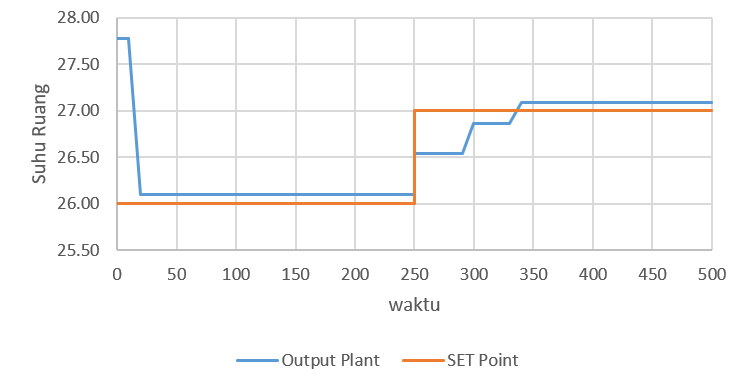
\includegraphics[width=0.75\textwidth]{figures/SimulinkSP3Td}
	\caption{Hasil Simulasi Sistem Kontrol untuk Suhu Ruang SP3}
	\label{fig:5:SimulinkSP3Td}
\end{figure}

\begin{figure}[!h]
	\centering
	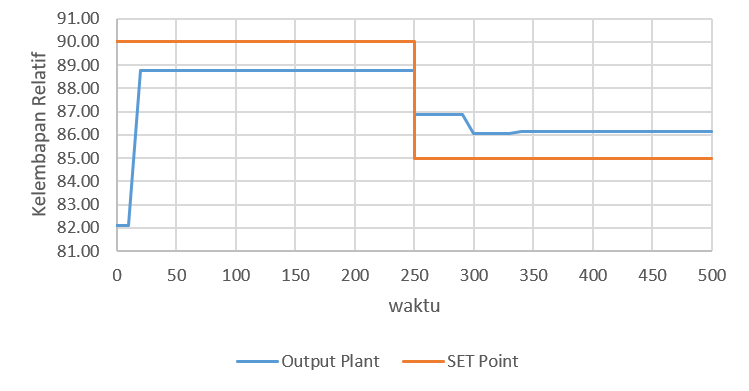
\includegraphics[width=0.75\textwidth]{figures/SimulinkSP3RH}
	\caption{Hasil Simulasi Sistem Kontrol untuk Kelembapan Relatif SP3}
	\label{fig:5:SimulinkSP3RH}
\end{figure}

\begin{figure}[!h]
	\centering
	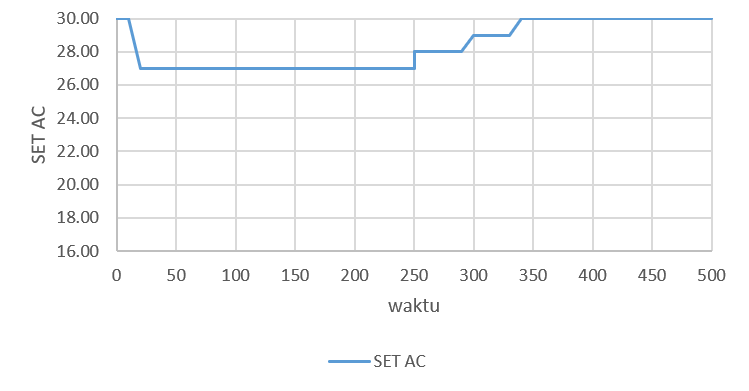
\includegraphics[width=0.75\textwidth]{figures/SimulinkSP3AC}
	\caption{Nilai MV SET AC SP3}
	\label{fig:5:SimulinkSP3AC}
\end{figure}

\begin{figure}[!h]
	\centering
	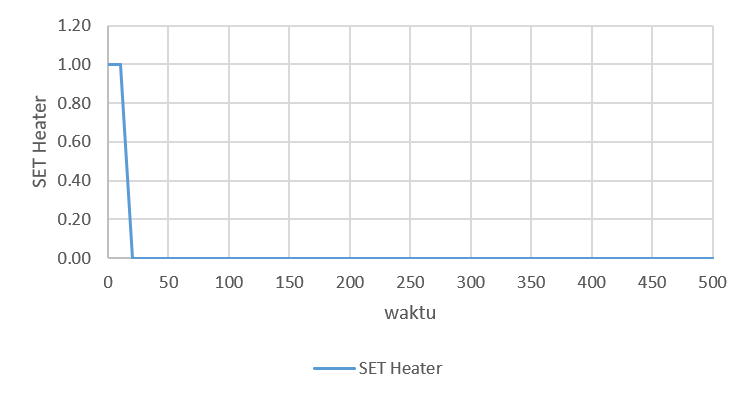
\includegraphics[width=0.75\textwidth]{figures/SimulinkSP3HT}
	\caption{Nilai MV SET Heater SP3}
	\label{fig:5:SimulinkSP3HT}
\end{figure}

Hasil simulasi dengan variasi SET POINT SP1, SP2, dan SP3 menunjukan bahwa sistem kontrol memiliki kinerja yang cukup baik dan sudah dapat mengikuti nilai SET POINT yang diinginkan.